\documentclass[12 pt]{article}
\usepackage[utf8]{inputenc}
\usepackage{matlab-prettifier}
\usepackage[portuguese]{babel}
\usepackage{indentfirst}
\usepackage{graphicx}
\usepackage{float}
\usepackage{subcaption}
\usepackage[font=small,labelfont=bf]{caption}
\definecolor{mygreen}{RGB}{28,172,0} % color values Red, Green, Blue
\definecolor{myyellow}{rgb}{1.0, 1.0, 0.8}
\usepackage{mathtools}
\usepackage{multirow}
\usepackage{comment}
\usepackage{xcolor}
\usepackage{colortbl}
\usepackage[normalem]{ulem}               % to striketrhourhg text
\usepackage{amsmath}
\usepackage{amsfonts}
\usepackage{hyperref}
\usepackage{tcolorbox}
\newcommand\redout{\bgroup\markoverwith
{\textcolor{red}{\rule[0.5ex]{2pt}{0.8pt}}}\ULon}
\renewcommand{\lstlistingname}{Código}% Listing -> Algorithm
\renewcommand{\lstlistlistingname}{Lista de \lstlistingname s}% List of Listings -> List of Algorithms

\usepackage[top=3cm,left=2cm,bottom=2cm, right=2cm]{geometry}
\usepackage{tikz}
\usetikzlibrary{decorations.pathreplacing}


% Configuração para destacar a sintaxe do Python
\lstset{ 
    language=Python,                     % A linguagem do código
    backgroundcolor=\color{myyellow}, % A cor do fundo 
    basicstyle=\ttfamily\footnotesize,   % O estilo do texto básico
    keywordstyle=\color{blue},           % Cor das palavras-chave
    stringstyle=\color{red},             % Cor das strings
    commentstyle=\color{mygreen},          % Cor dos comentários
    numbers=left,                        % Números das linhas à esquerda
    numberstyle=\tiny\color{gray},       % Estilo dos números das linhas
    stepnumber=1,                        % Número de linhas entre os números das linhas
    frame=single,                        % Moldura ao redor do código
    breaklines=true,                     % Quebra automática das linhas longas
    captionpos=t,                        % Posição da legenda
    showstringspaces=false               % Não mostra espaços em branco nas strings
    extendedchars=true,
    literate={º}{{${ }^{\underline{o}}$}}1 {á}{{\'a}}1 {à}{{\`a}}1 {ã}{{\~a}}1 {é}{{\'e}}1 {É}{{\'E}}1 {ê}{{\^e}}1 {ë}{{\"e}}1 {í}{{\'i}}1 {ç}{{\c{c}}}1 {Ç}{{\c{C}}}1 {õ}{{\~o}}1 {ó}{{\'o}}1 {ô}{{\^o}}1 {ú}{{\'u}}1 {â}{{\^a}}1 {~}{{$\sim$}}1
}


\title{%
\textbf{\huge Universidade Federal do Rio de Janeiro} \par
\textbf{\LARGE Instituto Alberto Luiz Coimbra de Pós-Graduação e Pesquisa de Engenharia} \par


\includegraphics[width=8cm]{COPPE UFRJ.png} \par

\textbf{Programa de Engenharia de Sistemas e Computação} \par

CPS863 - Aprendizado de Máquina  \par

Prof. Dr. Edmundo de Souza e Silva (PESC/COPPE/UFRJ)\par

\vspace{1\baselineskip}
\textbf{\textit{Lista de Exercícios 2}} \par
}

\author{Luiz Henrique Souza Caldas\\email: lhscaldas@cos.ufrj.br}

\date{\today}

\begin{document}
\maketitle

\section*{Questão 1 - HMM}

Considere o robô da lista anterior, que pode se mover pelos quadrados da figura abaixo.

\begin{figure}[H]
    \centering
    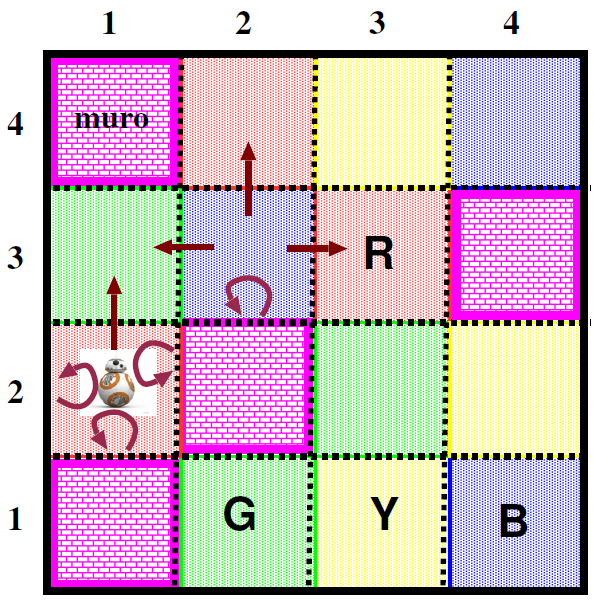
\includegraphics[width=0.5\textwidth]{fig/enunciado_q1.png}
    \caption{Robô andando por um ambiente}
    \label{fig:q1}
\end{figure}   

Para tentar melhorar a previsibilidade de se detectar a posição do robô da Figura \ref{fig:q1} sensores são colocados no ambiente onde o robô circula. Há 4 tipos de sensores (\textbf{R, B, Y, G}), conforme mostrado na Figura \ref{fig:q1}. Quando o robô está em qualquer um dos quadrados, o respectivo sensor emite um sinal (para um receptor) com a letra igual ao tipo do sensor. Entretanto, os sensores não são perfeitos e podem emitir um sinal errado com probabilidade 0.1. Por exemplo, quando o robô está num dos quadrados azuis, emite um sinal b com probabilidade 0.9, ou um dos restantes sinais r ou y ou g, com probabilidade 0.1/3. Como outro exemplo, suponha que o robô esteja na posição inicial conforme mostrado na Figura \ref{fig:q1}. Em 3 unidades de tempo, uma possível sequência de sinais recebidos poderiam ser \textbf{r g b}, se o robô for para norte e depois para leste. Entretanto, mesmo com o mesmo movimento, os sinais recebidos poderiam ser também \textbf{r g g} ou \textbf{b b b}, etc.

Seu objetivo é determinar a posição do robô, a partir dos sinais recebidos dos sensores.

\begin{itemize}
    \item \textbf{Explique como você fará uma HMM que possa permitir prever a posição do robô a partir dos sinais recebidos.}
    \begin{tcolorbox}[title=Resposta:]

    \begin{enumerate}
        \item \textbf{Estados:} Assim como no problema da lista anterior, os estados são as posições possíveis do robô, com a diferença de que agora os estados não podem ser diretamente observáveis. Para facilitar a notação, os estados foram numerados em ordem crescente da esquerda para a direita e de cima para baixo. Assim, o antigo estado (1,1) passou a se chamar $S_1$, (1,2) passou a se chamar $S_2$ e assim por diante. O modelo da Cadeia de Markov pode sewr visto na figura \ref{fig:cadeia_markov}.
        \item \textbf{Observações:} As observações são as emissões dos sensores, formadas pelos símbolos \textbf{R, B, Y, G}. 
        \item \textbf{Matriz de transição:} A matriz de transição é a mesma da lista anterior, com as probabilidades de transição entre os estados. Nesta lista foi utilizada a letra $A$ para representar a matriz de transição, seguindo a simbologia de Rabiner (1989) \cite{Rabiner1989}. A matriz $A$ é mostrada na tabela \ref{tab:matriz_transicao_a}.
        \item \textbf{Matriz de emissão:} A matriz de emissão é a probabilidade de cada estado emitir cada uma das observações. Cada estado tem uma probabilidade de 0.9 de emitir a cor dele mesmo e 0.1 de emitir qualquer outra cor ($0.1/3 \approx 0.0333 $ para cada cor). Os estados proibidos (rosa) possuem probabilidade de emissão 0 para todos os símbolos. A matriz de emissão é mostrada na tabela \ref{tab:matriz_emissao_b}.
        \item \textbf{Probabilidade inicial:} O vetor de probabilidades iniciais (renomeado para $\pi$ pelo mesmo motivo da matriz de transição) é o mesmo da lista anterior, com a probabilidade 1 do robô começar no estado $S_5$ (posição 2,1) $\pi_5=1$ e nula para os demais estados.
    \end{enumerate}

    \end{tcolorbox}

    \begin{figure}[H]
        \centering
        \begin{tikzpicture}[->, >=stealth, node distance=2cm, auto]
        
        % Define nodes with inverted y-axis and two-digit labels
        \node[state] (11) at (0,0) {$S_1$};
        \node[state] (12) [right=of 11] {$S_2$};
        \node[state] (13) [right=of 12] {$S_3$};
        \node[state] (14) [right=of 13] {$S_4$};
            
        \node[state] (21) [above=of 11] {$S_5$};
        \node[state] (22) [above=of 12] {$S_6$};
        \node[state] (23) [above=of 13] {$S_7$};
        \node[state] (24) [above=of 14] {$S_8$};
            
        \node[state] (31) [above=of 21] {$S_9$};
        \node[state] (32) [above=of 22] {$S_{10}$};
        \node[state] (33) [above=of 23] {$S_{11}$};
        \node[state] (34) [above=of 24] {$S_{12}$};
            
        \node[state] (41) [above=of 31] {$S_{13}$};
        \node[state] (42) [above=of 32] {$S_{14}$};
        \node[state] (43) [above=of 33] {$S_{15}$};
        \node[state] (44) [above=of 34] {$S_{16}$};


        % Transitions for node (1,2)
        \path (12) edge [loop below] node {0.75} (12) % Combined loop for south, west, and north (bottom border, wall at (1,1), wall at (2,2))
        edge[bend left] node[above] {0.25} (13);

        % Transitions for node (1,3)
        \path (13) edge [loop below] node {0.25} (13) % Loop for south (bottom border)
        edge[bend left] node[below] {0.25} (12)
        edge[bend left] node[above] {0.25} (14)
        edge[bend left] node[above] {0.25} (23);

        % Transitions for node (1,4)
        \path (14) edge [loop right] node {0.50} (14) % Combined loop for east and south (right border, bottom border)
        edge[bend left] node[below] {0.25} (13)
        edge[bend left] node[right] {0.25} (24);

        % Transitions for node (2,1)
        \path (21) edge [loop right] node {0.75} (21) % Combined loop for west, south, and east (left border, wall at (1,1), wall at (1,2))
        edge[bend left] node[above] {0.25} (31);

        % Transitions for node (2,3)
        \path (23) edge[bend left] node[below] {0.25} (13)
        edge [loop left] node {0.25} (23) % Loop for west (wall at (2,2))
        edge[bend left] node[above] {0.25} (24)
        edge[bend left] node[right] {0.25} (33);

        % Transitions for node (2,4)
        \path (24) edge [loop right] node {0.50} (24) % Combined loop for east and north (right border, wall at (3,4))
        edge[bend left] node[below] {0.25} (14)
        edge[bend left] node[below] {0.25} (23);

        % Transitions for node (3,1)
        \path (31) edge [loop left] node {0.50} (31) % Combined loop for west and north (left border, wall at (4,1))
        edge[bend left] node[below] {0.25} (21)
        edge[bend left] node[above] {0.25} (32);

        % Transitions for node (3,2)
        \path (32) edge[loop below] node {0.25} (32) % Loop for south (wall at (2,2))
        edge[bend left] node[below] {0.25} (31)
        edge[bend left] node[above] {0.25} (33)
        edge[bend left] node[right] {0.25} (42);

        % Transitions for node (3,3)
        \path (33) edge[bend left] node[below] {0.25} (23)
        edge[bend left] node[below] {0.25} (32)
        edge[loop right] node {0.25} (33) % Loop for east (wall at (3,4))
        edge[bend left] node[right] {0.25} (43);

        % Transitions for node (4,2)
        \path (42) edge [loop above] node {0.50} (42) % Combined loop for north and west (top border, wall at (4,1))
        edge[bend left] node[below] {0.25} (32)
        edge[bend left] node[above] {0.25} (43);

        % Transitions for node (4,3)
        \path (43) edge [loop above] node {0.25} (43) % Loop for north (top border)
        edge[bend left] node[below] {0.25} (33)
        edge[bend left] node[below] {0.25} (42)
        edge[bend left] node[above] {0.25} (44);

        % Transitions for node (4,4)
        \path (44) edge [loop right] node {0.75} (44) % Combined loop for east, north, and south (right border, top border, wall at (3,4))
        edge[bend left] node[below] {0.25} (43);
        
        \end{tikzpicture}
        \caption{Cadeia de Markov representando o movimento do robô no ambiente.}
        \label{fig:cadeia_markov}
        \end{figure}


        \begin{table}[H]
            \centering
            \resizebox{0.9\textwidth}{!}{
                \begin{tabular}{c|cccccccccccccccc}
                      & $S_1$ & $S_2$ & $S_3$ & $S_4$ & $S_5$ & $S_6$ & $S_7$ & $S_8$ & $S_9$ & $S_{10}$ & $S_{11}$ & $S_{12}$ & $S_{13}$ & $S_{14}$ & $S_{15}$ & $S_{16}$ \\
                    \hline
                    $S_1$ & 0    & 0    & 0    & 0    & 0    & 0    & 0    & 0    & 0    & 0    & 0    & 0    & 0    & 0    & 0    & 0 \\
                    $S_2$ & 0    & 0.75 & 0.25 & 0    & 0    & 0    & 0    & 0    & 0    & 0    & 0    & 0    & 0    & 0    & 0    & 0 \\
                    $S_3$ & 0    & 0.25 & 0.25 & 0.25 & 0    & 0    & 0.25 & 0    & 0    & 0    & 0    & 0    & 0    & 0    & 0    & 0 \\
                    $S_4$ & 0    & 0    & 0.25 & 0.50 & 0    & 0    & 0    & 0.25 & 0    & 0    & 0    & 0    & 0    & 0    & 0    & 0 \\
                    $S_5$ & 0    & 0    & 0    & 0    & 0.75 & 0    & 0    & 0    & 0.25 & 0    & 0    & 0    & 0    & 0    & 0    & 0 \\
                    $S_6$ & 0    & 0    & 0    & 0    & 0    & 0    & 0    & 0    & 0    & 0    & 0    & 0    & 0    & 0    & 0    & 0 \\
                    $S_7$ & 0    & 0    & 0.25 & 0    & 0    & 0    & 0.25 & 0.25 & 0    & 0    & 0.25 & 0    & 0    & 0    & 0    & 0 \\
                    $S_8$ & 0    & 0    & 0    & 0.25 & 0    & 0    & 0.25 & 0.50 & 0    & 0    & 0    & 0    & 0    & 0    & 0    & 0 \\
                    $S_9$ & 0    & 0    & 0    & 0    & 0.25 & 0    & 0    & 0    & 0.50 & 0.25 & 0    & 0    & 0    & 0    & 0    & 0 \\
                    $S_{10}$ & 0    & 0    & 0    & 0    & 0    & 0    & 0    & 0    & 0.25 & 0.25 & 0.25 & 0    & 0    & 0.25 & 0    & 0 \\
                    $S_{11}$ & 0    & 0    & 0    & 0    & 0    & 0    & 0.25 & 0    & 0    & 0.25 & 0.25 & 0    & 0    & 0    & 0.25 & 0 \\
                    $S_{12}$ & 0    & 0    & 0    & 0    & 0    & 0    & 0    & 0    & 0    & 0    & 0    & 0    & 0    & 0    & 0    & 0 \\
                    $S_{13}$ & 0    & 0    & 0    & 0    & 0    & 0    & 0    & 0    & 0    & 0    & 0    & 0    & 0    & 0    & 0    & 0 \\
                    $S_{14}$ & 0    & 0    & 0    & 0    & 0    & 0    & 0    & 0    & 0    & 0.25 & 0    & 0    & 0    & 0.50 & 0.25 & 0 \\
                    $S_{15}$ & 0    & 0    & 0    & 0    & 0    & 0    & 0    & 0    & 0    & 0    & 0.25 & 0    & 0    & 0.25 & 0.25 & 0.25 \\
                    $S_{16}$ & 0    & 0    & 0    & 0    & 0    & 0    & 0    & 0    & 0    & 0    & 0    & 0    & 0    & 0    & 0.25 & 0.75 \\
                \end{tabular}
            }
            \caption{Matriz de Transição A}
            \label{tab:matriz_transicao_a}
        \end{table}

        \begin{table}[H]
            \centering
            \resizebox{0.9\textwidth}{!}{
                \begin{tabular}{c|cccccccccccccccc}
                      & $S_1$ & $S_2$ & $S_3$ & $S_4$ & $S_5$ & $S_6$ & $S_7$ & $S_8$ & $S_9$ & $S_{10}$ & $S_{11}$ & $S_{12}$ & $S_{13}$ & $S_{14}$ & $S_{15}$ & $S_{16}$ \\
                    \hline
                    R (Vermelho) & 0     & 0.0333  & 0.0333  & 0.0333  & 0.9000  & 0       & 0.0333  & 0.0333  & 0.0333  & 0.0333  & 0.9000  & 0       & 0      & 0.9000  & 0.0333  & 0.0333 \\
                    B (Azul)     & 0     & 0.0333  & 0.0333  & 0.9000  & 0.0333  & 0       & 0.0333  & 0.0333  & 0.0333  & 0.9000  & 0.0333  & 0       & 0      & 0.0333  & 0.0333  & 0.9000 \\
                    Y (Amarelo)  & 0     & 0.0333  & 0.9000  & 0.0333  & 0.0333  & 0       & 0.0333  & 0.9000  & 0.0333  & 0.0333  & 0.0333  & 0       & 0      & 0.0333  & 0.9000  & 0.0333 \\
                    G (Verde)    & 0     & 0.9000  & 0.0333  & 0.0333  & 0.0333  & 0       & 0.9000  & 0.0333  & 0.9000  & 0.0333  & 0.0333  & 0       & 0      & 0.0333  & 0.0333  & 0.0333 \\
                \end{tabular}
            }
            \caption{Matriz de Emissão \( B \)}
            \label{tab:matriz_emissao_b}
        \end{table}
    
    \item \textbf{Suponha que o receptor de sinais tenha recebido a sequência}
    r r y r y r b g b r y y g b. Qual a probabilidade desta sequência ocorrer? Explique e implemente o algoritmo necessário para responder a pergunta.
    \begin{tcolorbox}[title=Resposta:]
        Assim como no problema 1 de \cite{Rabiner1989}, devemos utilizar a etapa forward do algoritmo forward-backward para calcular a probabilidade da sequência de observações. Esta etapa pode ser dividida em 3 passos:

        \begin{itemize}
            \item Inicialização: a variavel \( \alpha_1(i) \) é calculada para cada estado \( i \) como a probabilidade de estar no estado \( i \) e emitir a observação \( O_1 \).
            \begin{equation}
                \alpha_1(i) = \pi_i b_i(O_1)
            \end{equation}
            \item Indução: a variável \( \alpha_t(i) \) é calculada para cada estado \( i \) como a probabilidade de estar no estado \( i \) e emitir a observação \( O_t \) dado que a sequência de observações até o tempo \( t-1 \) foi observada.
            \begin{equation}
                \alpha_t(i) = P(O_1, O_2, \ldots, O_t, q_t = S_i | \lambda) = \sum_{j=1}^{N} \alpha_{t-1}(j) a_{ji} b_i(O_t)
            \end{equation} 
            \item Termino: a probabilidade total da sequência de observações é dada por:
            \begin{equation}
                P(O |  \lambda) = \sum_{i=1}^{N} \alpha_T(i)
            \end{equation}
        \end{itemize}

        onde \(  \lambda \) é o modelo, \( N \) é o número de estados, \( \pi_i \) é a probabilidade inicial de estar no estado \( i \), \( a_{ji} \) é a probabilidade de transição do estado \( j \) para o estado \( i
        \) e \( b_i(O_t) \) é a probabilidade de emitir a observação \( O_t \) no estado \( i \).

        Para isso, foi implementada em python a classe HMM, que recebe as matrizes \( A \) e \( B \) ao ser inicializada e contém os métodos forward para calcular a probabilidades \(\alpha\) de uma dada sequência e método P\_obs, que calcula a probabilidade total daquela observação, para um dado alpha. O código fonte da classe HMM pode ser visto no código \ref{lst:hmm}.
    \end{tcolorbox}

    \begin{lstlisting}[language=Python, caption=Classe HMM, label={lst:hmm}]
        class HMM:
            def __init__(self, A, B, pi):
                """
                Inicializa o modelo HMM.
                
                :param A: Matriz de transição de estados (N x N)
                :param B: Matriz de emissão de observações (N x M)
                :param pi: Vetor de probabilidades iniciais (1 x N)
                """
                self.A = A  # Matriz de transição
                self.B = B  # Matriz de emissão
                self.pi = pi  # Probabilidades iniciais

            def forward(self, O):
                """
                Calcula o alpha para todos os estados e tempos para uma sequência O.

                :param O: Sequência de observações (lista de índices das observações)
                :return: Matriz alpha (T x N)
                """
                N = len(self.pi)  # Número de estados
                T = len(O)  # Comprimento da sequência de observações

                # Inicialização
                alpha = np.zeros((T, N))
                alpha[0, :] = self.pi * self.B[:, O[0]]

                # Recursão
                for t in range(1, T):
                    for j in range(N):
                        alpha[t, j] = np.sum(alpha[t - 1, :] * self.A[:, j]) * self.B[j, O[t]]

                return alpha

            def P_obs(self, alpha):
                """
                Calcula a probabilidade da sequência de observações, dado o modelo.
                
                :param alpha: Matriz alpha (T x N) calculada pelo método forward
                :return: Probabilidade da sequência de observações
                """
                return np.sum(alpha[-1, :])
    \end{lstlisting}

    \begin{tcolorbox}[title=Resposta (continuação):]
        O resultado obtido para a sequência \( r r y r y r b g b r y y g b \) foi:
        \begin{equation}
            P(O |  \lambda) = 4.3021 \times 10^{-10}
        \end{equation}

        A probabilidade obtida foi um valor muito pequeno, porém esse resultado é esperado. Isso ocorre pois:
        \begin{itemize}
            \item O robô possui muitas possibilidades de movimento;
            \item A sequência de observações é relativamente longa;
            \item A probabilidade de emissão de uma cor diferente da esperada para um estado é de $0.0333$ para cada cor.
        \end{itemize}
        
        Juntos, esses fatores contribuem para que o resultado seja um valor muito pequeno.
    \end{tcolorbox}

    \item \textbf{Repita o item anterior para a sequência r b y r g r b g b r y y g b. (Obviamente não precisa reimplementar o algoritmo!)}
    \begin{tcolorbox}[title=Resposta:]
        Utilizando o mesmo código do item anterior, o resultado obtido para a sequência \( r b y r g r b g b r y y g b \) foi:
        \begin{equation}
            P(O |  \lambda) = 1.0925 \times 10^{-10}
        \end{equation}

        O resultado obtido foi cerca de 4 vezes menor que o obtido na sequência anterior, mostrando que essa sequencia é menos provável de ocorrer.
    \end{tcolorbox}

    \item \textbf{Para a primeira sequência acima, qual o quadrado mais provável onde estará o robô na última posição (isto é, o quadrado de onde foi emitido o último sinal)? Explique e implemente o algoritmo necessário.}
    \begin{tcolorbox}[title=Resposta:]
        A soluçáo para este item esta na parte inicial do problema 2 de \cite{Rabiner1989}, onde a variável $\gamma = P (q_t = S_i | O, \lambda)$ é definida como a probabilidade de estar no estado $S_i$ no tempo $t$ dado o modelo $\lambda$ e a sequência de observações $O$, sendo dada por:
        \begin{equation}
            \gamma_t(i) = P(q_t = S_i | O, \lambda) = \frac{\alpha_t(i) \beta_t(i)}{P(O | \lambda)} = \frac{\alpha_t(i) \beta_t(i)}{\sum_{j=1}^{N} \alpha_t(j) \beta_t(j)}
        \end{equation}

        onde $\beta_t(i)$ é a probabilidade de observar a sequência $O_{t+1}, O_{t+2}, \ldots, O_T$ dado que o sistema está no estado $S_i$ no tempo $t$, sendo calculada na etapa backward do algoritmo forward-backward:

        \begin{equation}
            \beta_t(i) = P(O_{t+1}, O_{t+2}, \ldots, O_T | q_t = S_i, \lambda) = \sum_{j=1}^{N} a_{ij} b_j(O_{t+1}) \beta_{t+1}(j)
        \end{equation}

        Para calcular o estado final mais provável, foram implementados os métodos backward e gamma, que calculam as matrizes $\beta$ e $\gamma$, respectivamente. Além disso, foi implementado o método end\_state, que recebe a matriz gamma e retorna o estado mais provável na última observação e o valor da probabilidade para aquele estado ser o último. O código fonte dos métodos backward, gamma e end\_state pode ser visto no código \ref{lst:end_state}.
    
    \end{tcolorbox}    
    
    \begin{lstlisting}[language=Python, caption={backward, gamma e end\_state}, label={lst:end_state}]
    def backward(self, O):
        """
        Calcula o beta para todos os estados e tempos para uma sequência O.

        :param O: Sequência de observações (lista de índices das observações)
        :return: Matriz beta (T x N)
        """
        N = len(self.pi)
        T = len(O)

        # Inicialização
        beta = np.zeros((T, N))
        beta[-1, :] = 1

        # Recursão
        for t in range(T - 2, -1, -1):
            for i in range(N):
                beta[t, i] = np.sum(self.A[i, :] * self.B[:, O[t + 1]] * beta[t + 1, :])

        return beta
    
    def gamma(self, alpha, beta):
        """
        Calcula a matriz gamma para todos os estados e tempos para uma sequência O.
        
        :param alpha: Matriz alpha (T x N) calculada pelo método forward
        :param beta: Matriz beta (T x N) calculada pelo método backward
        :return: Matriz gamma (T x N)
        """
        return alpha * beta / np.sum(alpha * beta, axis=1).reshape(-1, 1)

    def end_state(self, gamma):
            """
            Calcula o estado mais provável na última observação.
            
            :param gamma: Matriz gamma (T x N) calculada pelo método gamma
            :return: Estado mais provável na última observação
            """
            end_state = np.argmax(gamma[-1, :])
            P_end_state = gamma[-1, end_state]
            state_map = {0: 'S1', 1: 'S2', 2: 'S3', 3: 'S4', 4: 'S5', 5: 'S6', 6: 'S7', 7: 'S8', 8: 'S9', 9: 'S10', 10: 'S11', 11: 'S12', 12: 'S13', 13: 'S14', 14: 'S15', 15: 'S16'}
            return state_map[end_state], P_end_state        
    \end{lstlisting}

    \begin{tcolorbox}[title=Resposta (continuação):]
        Executando o código acima, o resultado obtido para a sequência \( r r y r y r b g b r y y g b \) foi que o estado mais provável na última observação é o estado \( S_{11} \) (X=3, Y=3), com probabilidade de $0.6055$.
    \end{tcolorbox}

    \item \textbf{Para a segunda sequência acima, qual o quadrado mais provável onde estará o robô?}
    
    \begin{tcolorbox}[title=Resposta:]
        Executando o mesmo código do item anterior, o resultado obtido para a sequência \( r b y r g r b g b r y y g b \) foi que o estado mais provável na última observação também é o estado \( S_{11} \) (X=3, Y=3), porém com probabilidade de $0.6092$, muito próxima da probabilidade obtida na sequência anterior.
    \end{tcolorbox}

    \item \textbf{Para a primeira sequência acima, qual o caminho mais provável percorrido pelo robô? Explique o algoritmo usado, mas não precisa implementar. Use uma biblioteca de Python ou outra linguagem preferida.}
    \begin{tcolorbox}[title=Resposta:]
        Com base no problema 2 de \cite{Rabiner1989}, o caminho mais provável percorrido pelo robô é obtido através do algoritmo de Viterbi, que calcula a sequência de estados mais provável para uma dada sequência de observações. O algoritmo de Viterbi é é baseado no cálculo da variável \( \delta_t(i) \), que é a probabilidade da sequência mais provável de estados até o tempo \( t \) e que termina no estado \( i \), sendo dada por:
        \begin{equation}
            \delta_{t}(i) = max_{q_1, q_2, \ldots, q_t} [P(q_1, q_2, \ldots, q_t = S_i, O_1, O_2, \ldots, O_{t} | \lambda)]
        \end{equation}

        A cada passo também é calculada a variável \( \psi_t(i) \), que é o estado anterior mais provável para o estado \( i \) no tempo \( t \).

        \begin{itemize}
            \item Inicialização: a variável \( \delta_1(i) \) é calculada para cada estado \( i \) como a probabilidade de estar no estado \( i \) e emitir a observação \( O_1 \).
            \begin{equation}
                \delta_1(i) = \pi_i b_i(O_1)
            \end{equation}
            e
            \begin{equation}
                \psi_1(i) = 0
            \end{equation}
            \item Recursão: a variável \( \delta_t(i) \) é calculada para cada estado \( i \) como a probabilidade de estar no estado \( i \) e emitir a observação \( O_t \) dado que a sequência de observações até o tempo \( t-1 \) foi observada. A variável \( \psi_t(i) \) é calculada como o estado anterior mais provável para o estado \( i \).
            \begin{equation}
                \delta_t(j) = max_{1 \leq i \leq N} [\delta_{t-1}(i) a_{ij}] b_j(O_t)
            \end{equation}
            e
            \begin{equation}
                \psi_t(j) = argmax_{1 \leq i \leq N} [\delta_{t-1}(i) a_{ij}]
            \end{equation}
        \item Finalização: O estado final mais provável e a sua probabilide são calculados.
        \begin{equation}
            q_T^* = argmax_{1 \leq i \leq N} \delta_T(i)
        \end{equation}
        e
        \begin{equation}
            P^* = max_{1 \leq i \leq N} \delta_T(i)
        \end{equation}
        \item Retrocesso: O caminho mais provável é obtido retrocedendo a partir do estado final mais provável, utilizando os valores de \( \psi_t(i) \) calculados na etapa de recursão.
        \begin{equation}
            q_t^* = \psi_{t+1}(q_{t+1}^*)
        \end{equation}

        Foi implementado na classe HMM o método viterbi, que recebe a sequência de observações e retorna o caminho mais provável percorrido pelo robô. O código fonte do método viterbi pode ser visto no código \ref{lst:viterbi}.
        \end{itemize}

        \end{tcolorbox}

        \begin{lstlisting}[language=Python, caption={viterbi}, label={lst:viterbi}]
                def viterbi(self, O):
                    # inicialização
                    N = len(self.pi)
                    T = len(O)
                    delta = np.zeros((T, N))
                    psi = np.zeros((T, N), dtype=int)
                    delta[0, :] = self.pi * self.B[:, O[0]]
                    psi[0, :] = 0

                    # recursão
                    for t in range(1, T):
                        for j in range(N):
                            delta[t, j] = np.max(delta[t - 1, :] * self.A[:, j]) * self.B[j, O[t]]
                            psi[t, j] = np.argmax(delta[t - 1, :] * self.A[:, j])
                    
                    # finalização
                    P_star = np.max(delta[-1, :])
                    q_star = np.argmax(delta[-1, :])

                    # reconstrução do caminho
                    path = [q_star]
                    for t in range(T - 1, 0, -1):
                        q_star = psi[t, q_star]
                        path.insert(0, q_star)

                    state_map = {0: 'S1', 1: 'S2', 2: 'S3', 3: 'S4', 4: 'S5', 5: 'S6', 6: 'S7', 7: 'S8', 8: 'S9', 9: 'S10', 10: 'S11', 11: 'S12', 12: 'S13', 13: 'S14', 14: 'S15', 15: 'S16'}
                    path = [state_map[state] for state in path]
                    return path, P_star
        \end{lstlisting}

        \begin{tcolorbox}[title=Resposta (continuação):]
            Executando o código acima, o resultado obtido para a sequência \( r r y r y r b g b r y y g b \) foi que a sequência de estados mais provável percorrida pelo robô foi: ['S5', 'S5', 'S5', 'S5', 'S5', 'S5', 'S9', 'S10', 'S11', 'S7', 'S8', 'S8', 'S7', 'S11'], com probabilidade de $8.3918 \times 10^{-11}$.

            Apesar de não ter sido pedido no item, o caminho mais provével para a segunda sequência, \( r b y r g r b g b r y y g b \), foi: ['S5', 'S9', 'S5', 'S5', 'S5', 'S5', 'S9', 'S10', 'S11', 'S7', 'S8', 'S8', 'S7', 'S11'], com probabilidade de $9.3242 \times 10^{-12}$.
        \end{tcolorbox}
    
\end{itemize}


\section*{Questão 2}

\subsection*{Definição da Cadeia de Markov}

A cadeia de Markov para este problema é definida pelos seguintes elementos:

\begin{enumerate}
    \item \textbf{Estados}: Representados pela tupla $(c, s)$, onde:
    \begin{itemize}
        \item $c$ é o número de clientes no sistema (limitado entre 0 e 8).
        \item $s$ é o número de servidores disponíveis (limitado entre 1 e 3).
    \end{itemize}

    \item \textbf{Ações}: As ações disponíveis em cada estado são:
    \begin{itemize}
        \item $-1$: Remover um servidor.
        \item $0$: Manter o número atual de servidores.
        \item $+1$: Adicionar um servidor (respeitando os limites).
    \end{itemize}

    \item \textbf{Transições}: Determinadas pelas probabilidades de chegada de novos clientes no final de cada intervalo de tempo:
    \begin{itemize}
        \item $p_0 = 0.4$: Probabilidade de 0 clientes chegarem.
        \item $p_2 = 0.2$: Probabilidade de 2 clientes chegarem.
        \item $p_4 = 0.4$: Probabilidade de 4 clientes chegarem.
    \end{itemize}
    A transição entre estados considera:
    \begin{itemize}
        \item Atendimento: $\min(c, s)$ clientes são atendidos no início de cada intervalo.
        \item Clientes restantes: Permanecem no sistema para o próximo intervalo.
        \item Restrições: O número total de clientes no sistema é limitado a 8.
    \end{itemize}

    \item \textbf{Ordem dos eventos}: Para cada intervalo de tempo, a ordem dos eventos considerada é:
    \begin{enumerate}[label=\roman*.]
        \item Atendimento de clientes.
        \item Adição/remoção de servidores.
        \item Chegada de clientes.
    \end{enumerate}

    \item \textbf{Recompensas}: A recompensa para cada transição é composta por:
    \begin{itemize}
        \item Ganho por cliente atendido: $T \cdot \min(c, s)$, com $T = 10$.
        \item Custo por servidor: $-R_s \cdot s'$, com $R_s = 5$.
        \item Penalidade por fila: $-R_q$ se $c' > 4$, caso contrário $0$, com $R_q = 10$.
        \item Penalidade por ociosidade: $-R_0$ por servidor não utilizado, max($s' - c', 0$), com $R_0 = 2$.
    \end{itemize}
    Onde $c$ e $s$ são os valores de clientes e servidores no estado atual e $c'$ e $s'$ são os valores no próximo estado.
\end{enumerate}

\subsection*{Solução por \textit{Value Iteration}}

Foi implemmentado em Python uma função que calcula a política ótima para a cadeia de Markov descrita. O código fonte está disponível no repositório indicado no final deste relatório, na pasta \texttt{lista\_6}, arquivo \texttt{value\_itaration.py}. O código principal, onde são definidas as probabilidades de transição e as recompensas, está disponível no arquivo \texttt{main.py}. O código segue o seguinte fluxo:

\begin{enumerate}
    \item Inicializa \( V[s] = 0 \) para todos os estados \( s \).
    \item Iterativamente calcula os valores \( V[s] \) para cada estado, atualizando-os com base na equação de Bellman:
    \[
    V(s) = \max_a \sum_{s', r} P(s', r \mid s, a) \cdot \left( r + \gamma \cdot V(s') \right).
    \]
    \item Em cada iteração, verifica a convergência comparando a maior mudança (\( \Delta \)) entre os valores antigos e novos. O loop termina quando \( \Delta < \theta \), o limiar definido.
    \item Após convergir, calcula a política ótima \( \pi^*(s) \) para cada estado, escolhendo a ação \( a \) que maximiza o valor esperado \( V(s) \):
    \[
    \pi^*(s) = \arg\max_a \sum_{s', r} P(s', r \mid s, a) \cdot \left( r + \gamma \cdot V(s') \right).
    \]
    \item Retorna a função de valor ótima \( V(s) \) e a política ótima \( \pi^*(s) \).
\end{enumerate}

Foi utilizado um fator de desconto $\gamma = 0.9$ e um limiar de convergência $\theta = 1e-6$. Para esses valores, a convergência ocorreu em 2457 iterações. A função de valor ótima calculada e a política ótima derivada dela são apresentadas na figura \ref{fig:value_iteration_policy_and_values}.
A variação de $\Delta$ ao longo das iterações é apresentada na figura \ref{fig:value_iteration_delta}.

\begin{figure}[H]
    \centering
    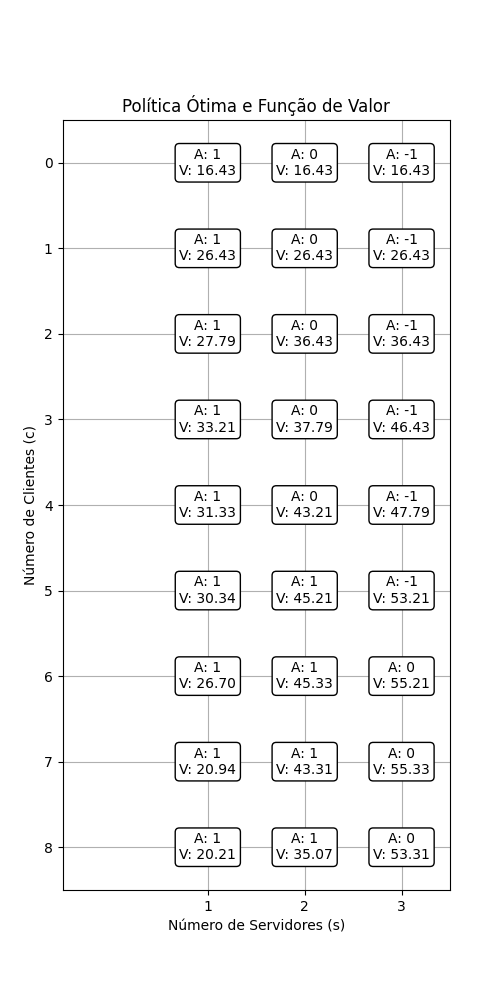
\includegraphics[width=0.5\textwidth]{fig/value_iteration_policy_and_values.png}
    \caption{Função de valor ótima e política ótima calculadas por \textit{Value Iteration}.}
    \label{fig:value_iteration_policy_and_values}
\end{figure}

\begin{figure}[H]
    \centering
    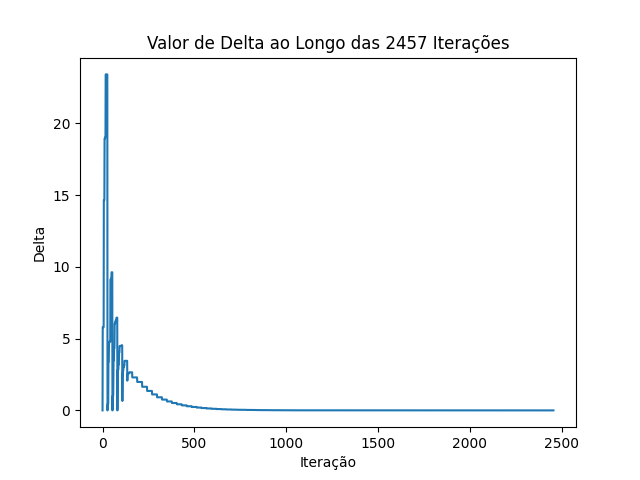
\includegraphics[width=0.5\textwidth]{fig/value_iteration_delta.png}
    \caption{Variação de $\Delta$ ao longo das iterações de \textit{Value Iteration}.}
    \label{fig:value_iteration_delta}
\end{figure}



\subsection*{Solução por \textit{Policy Iteration}}

Foi implementado em Python uma função que calcula a política ótima para a cadeia de Markov descrita. O código fonte está disponível no repositório indicado no final deste relatório, na pasta \texttt{lista\_6}, arquivo \texttt{policy\_itaration.py}. O código principal, onde são definidas as probabilidades de transição e as recompensas, está disponível no arquivo \texttt{main.py}. O código segue o seguinte fluxo:

\begin{enumerate}
    \item Inicializa uma política arbitrária \( \pi(s) = -1 \) e uma função de valor \( V(s) = 0 \) para todos os estados \( s \).
    \item \textbf{Etapa 1 - Avaliação da Política:}
    \begin{enumerate}
        \item Para cada estado \( s \), atualiza \( V(s) \) usando a equação:
        \[
        V(s) = \sum_{s',r} P(s', r \mid s, \pi(s)) \cdot \left( r + \gamma \cdot V(s') \right).
        \]
        \item Repete as atualizações até que a maior mudança em \( V(s) \) entre duas iterações seja menor que um limiar \( \theta \).
    \end{enumerate}
    \item \textbf{Etapa 2 - Melhoria da Política:}
    \begin{enumerate}
        \item Para cada estado \( s \), identifica a melhor ação \( a \) que maximiza o valor esperado:
        \[
        \pi(s) = \arg\max_a \sum_{s', r} P(s', r \mid s, a) \cdot \left( r + \gamma \cdot V(s') \right).
        \]
        \item Se a nova política \( \pi(s) \) for igual à política anterior para todos os estados, o algoritmo termina. Caso contrário, retorna à etapa de avaliação.
    \end{enumerate}
    \item Retorna a política ótima \( \pi^*(s) \) e a função de valor ótima \( V^*(s) \).
\end{enumerate}

Foi utilizado um fator de desconto $\gamma = 0.9$ e um limiar de convergência $\theta = 1e-6$. Para esses valores, a convergência ocorreu em 4 iterações do laço externo \textit{while principal}, porém foram contabiizadas um total de 5292 iterações internas da etapa de avaliação da política. A função de valor ótima calculada e a política ótima derivada dela são apresentadas na figura \ref{fig:policy_iteration_policy_and_values}. A variação de $\Delta$ ao longo das iterações é apresentada na figura \ref{fig:policy_iteration_delta}.

\begin{figure}[H]
    \centering
    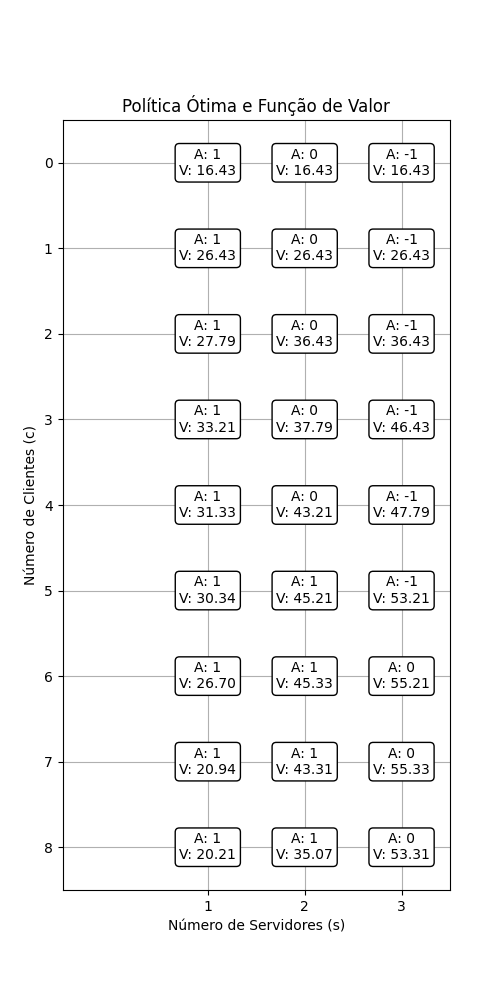
\includegraphics[width=0.5\textwidth]{fig/policy_iteration_policy_and_values.png}
    \caption{Função de valor ótima e política ótima calculadas por \textit{Policy Iteration}.}
    \label{fig:policy_iteration_policy_and_values}
\end{figure}

\begin{figure}[H]
    \centering
    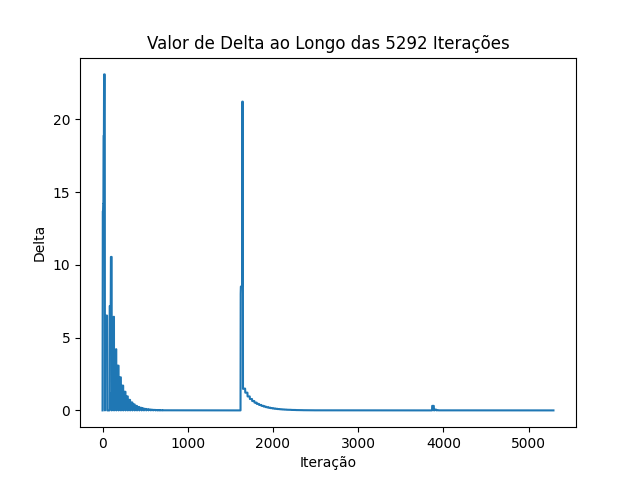
\includegraphics[width=0.5\textwidth]{fig/policy_iteration_delta.png}
    \caption{Variação de $\Delta$ ao longo das iterações de \textit{Policy Iteration}.}
    \label{fig:policy_iteration_delta}
\end{figure}

\subsection*{Q-Learning}

Foi implementado em Python um algoritmo de \textit{Q-Learning} para resolver o problema da cadeia de Markov descrita. O código fonte está disponível no repositório indicado no final deste relatório, na pasta \texttt{lista\_6}, arquivo \texttt{q\_learning.py}. O código principal, onde são definidas as probabilidades de transição e as recompensas, está disponível no arquivo \texttt{main.py}. Como o problema em questão não possui estado terminal, o algoritmo foi adaptado para, a cada epsódio, limitar o número de passos. Além disso, foi implementada uma classe \texttt{EnvironmentSimulator} para simular o ambiente, recebendo como entrada o estado atual e a ação tomada e retornando o próximo estado e a recompensa obtida. O código segue o seguinte fluxo:

\begin{enumerate}
    \item Inicializa \( Q(s, a) \) com zeros para todos os estados e ações.
    \item Para cada episódio:
    \begin{enumerate}
        \item Escolhe um estado inicial aleatório.
        \item Para cada passo no episódio:
        \begin{enumerate}
            \item Escolhe uma ação (usando política \( \epsilon \)-gulosa):
            \begin{itemize}
                \item Com probabilidade \( \epsilon \), escolhe uma ação aleatória (\textit{exploration}).
                \item Caso contrário, escolhe a ação que maximiza \( Q(s, a) \) (\textit{exploitation}).
            \end{itemize}
            \item Simula o ambiente com a ação escolhida para obter:
            \begin{itemize}
                \item O próximo estado \( s' \).
                \item A recompensa \( r \).
            \end{itemize}
            \item Atualiza \( Q(s, a) \) usando a equação de aprendizado por diferença temporal (TD):
            \[
            Q(s, a) \leftarrow Q(s, a) + \alpha \left[ r + \gamma \max_{a'} Q(s', a') - Q(s, a) \right]
            \]
            \item Atualiza o estado atual para \( s' \).
            \item Se atingir o número máximo de passos, termina o episódio.
        \end{enumerate}
        \item Após o episódio, calcula:
        \begin{itemize}
            \item A nova função de valor \( V(s) = \max_a Q(s, a) \).
            \item A mudança absoluta máxima \( \Delta V = \max_s |V_{\text{novo}}(s) - V(s)| \).
        \end{itemize}
        \item Atualiza \( V(s) \) e armazena \( \Delta V \) para análise de convergência.
    \end{enumerate}
    \item Deriva a política ótima \( \pi^*(s) \) escolhendo, para cada estado, a ação que maximiza \( Q(s, a) \).
    \item Retorna a política ótima \( \pi^*(s) \), a função de valor \( V(s) \), e a lista de \( \Delta V \) ao longo dos episódios.
\end{enumerate}

Foram utilizados os seguintes hiperparâmetros: fator de desconto \( \gamma = 0.9 \), taxa de aprendizado \( \alpha = 0.1 \), probabilidade de exploração \( \epsilon = 0.1 \), número de episódios \( 1000 \) e limite de passos por episódio \( 100 \). Como não há um critério de convergência, o algoritmo executa 100 mil iterações. A função de valor ótima calculada e a política ótima derivada dela são apresentadas na figura \ref{fig:q_learning_policy_and_values}. A variação de \( \Delta V \) ao longo dos episódios é apresentada na figura \ref{fig:q_learning_delta}.

\begin{figure}[H]
    \centering
    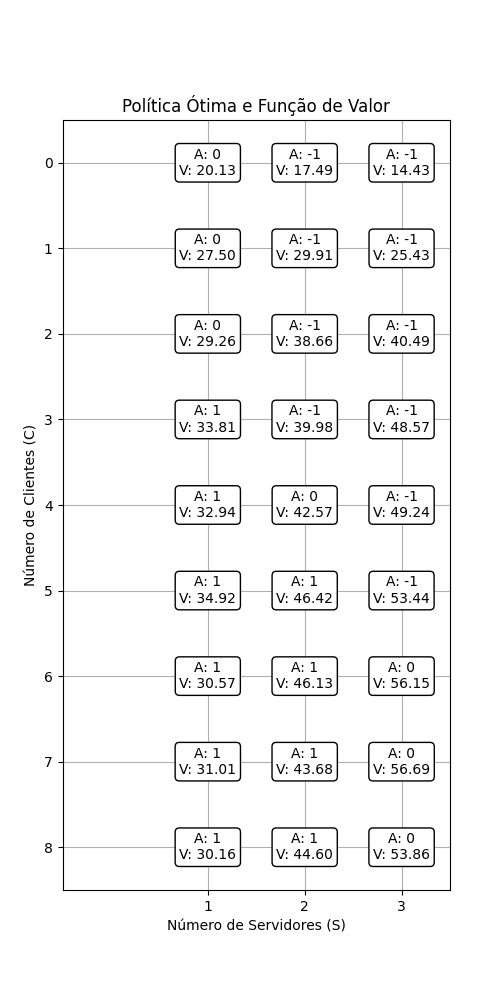
\includegraphics[width=0.5\textwidth]{fig/q_learning_policy_and_values.png}
    \caption{Função de valor ótima e política ótima calculadas por \textit{Q-Learning}.}
    \label{fig:q_learning_policy_and_values}
\end{figure}

\begin{figure}[H]
    \centering
    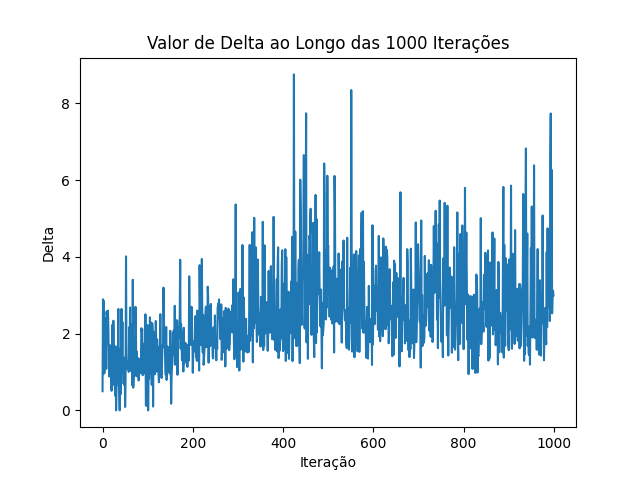
\includegraphics[width=0.5\textwidth]{fig/q_learning_delta.png}
    \caption{Variação de \( \Delta V \) ao longo dos episódios de \textit{Q-Learning}.}
    \label{fig:q_learning_delta}
\end{figure}

OBS: devido a aleatoriedade do algoritmo, e a falta de um estado terminal, não é possível observar uma convergência clara na figura \ref{fig:q_learning_delta}, como nos métodos anteriores. Entretanto é poss~ivel observar que os valores de \( V^* (s) \) para cada estado na figura \ref{fig:q_learning_policy_and_values} são próximos dos valores obtidos pelos métodos anteriores e as ações da política ótima também são semelhantes.

\subsection*{Comparação dos Métodos}

Abaixo vemos as figuras \ref{fig:value_iteration_policy_and_values}, \ref{fig:policy_iteration_policy_and_values} e \ref{fig:q_learning_policy_and_values} exibidas lado a lado.

% plot das figuras usando subfigure
\begin{figure}[H]
    \centering
    \begin{subfigure}{0.3\textwidth}
        \centering
        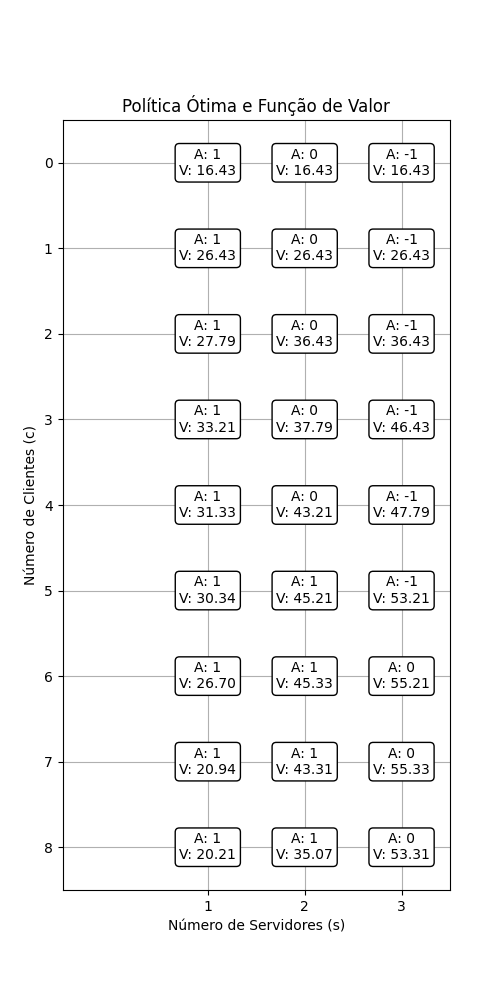
\includegraphics[width=\linewidth]{fig/value_iteration_policy_and_values.png}
        \caption{\textit{Value Iteration}}
    \end{subfigure}
    \begin{subfigure}{0.3\textwidth}
        \centering
        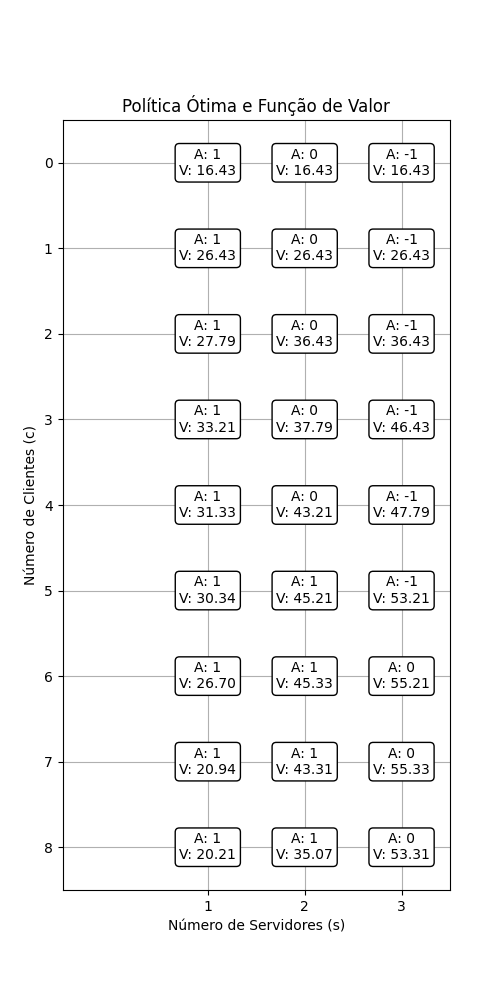
\includegraphics[width=\linewidth]{fig/policy_iteration_policy_and_values.png}
        \caption{\textit{Policy Iteration}}
    \end{subfigure}
    \begin{subfigure}{0.3\textwidth}
        \centering
        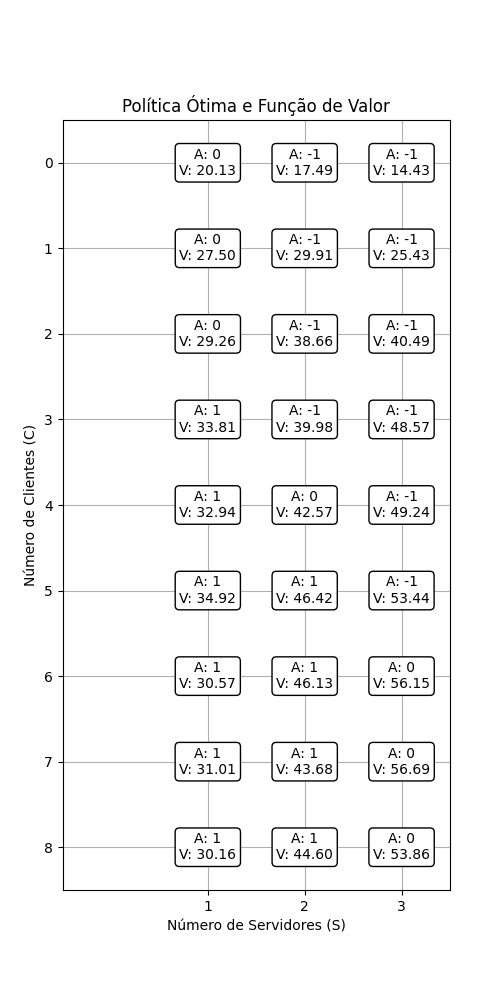
\includegraphics[width=\linewidth]{fig/q_learning_policy_and_values.png}
        \caption{\textit{Q-Learning}}
    \end{subfigure}
    \caption{Comparação das políticas e funções de valor ótimas calculadas pelos métodos.}
    \label{fig:comparison}
\end{figure}




\end{document}